\documentclass[usenames,dvipsnames,notes,11pt,aspectratio=169,hyperref={colorlinks=true, linkcolor=blue}]{beamer}
\usepackage{ifthen}
\usepackage{xcolor}
\usepackage{pgfplots}
\usepackage{amsmath}
\usepackage{centernot}
\usepackage{pifont}
\usepackage{tabularx}
\usepackage{makecell}
\usepackage{cuted}
\usepackage{booktabs}
\usepackage{array}
\usepackage{textcomp}
\usepackage{setspace}
\usepackage{xspace}
\usepackage{subcaption}
\usepackage{mdframed}
\usepackage{tikz}
\usepackage{pdfcomment}
%\newcommand{\pdfnote}[1]{\marginnote{\pdfcomment[icon=note]{#1}}}
\newcommand{\pdfnote}[1]{}

\usepackage{pgfpages}
%\setbeameroption{show notes on second screen}


\input ../beamer-style
\input ../std-macros
\input ../macros

\newcommand{\pt}{\partial}

\AtBeginSection[]
{
    \begin{frame}
        \frametitle{Table of Contents}
        \tableofcontents[currentsection]
    \end{frame}
}
\parskip=10pt

\title[CSCI-GA.2590]{Post-training of language models I}
\author[He He]{He He }
\institute[NYU]{
    
\includegraphics[height=1cm]{../figures/nyu-logo}\\
}
\date{March 12, 2025}

\begin{document}
\begin{frame}
\titlepage
\end{frame}

\section{Introduction}

\begin{frame}
    {Recap}
\begin{wideitemize}
    \item {\bf Pretraining} allows the model to acquire many capabilities from vast data
    \item Increasing {\bf compute} (data + parameters) {\it predictably} improves {\bf performance} (held-out perplexity)
    \item How to use a pretrained model for downstream tasks?
\end{wideitemize}
\end{frame}

% no weight update: prompting, in-context learning
% weight update: SFT, RLHF, LoRA 

\begin{frame}
    {Motivation}

    How do we tell the LM what we want to do?\\
    \begin{figure}
        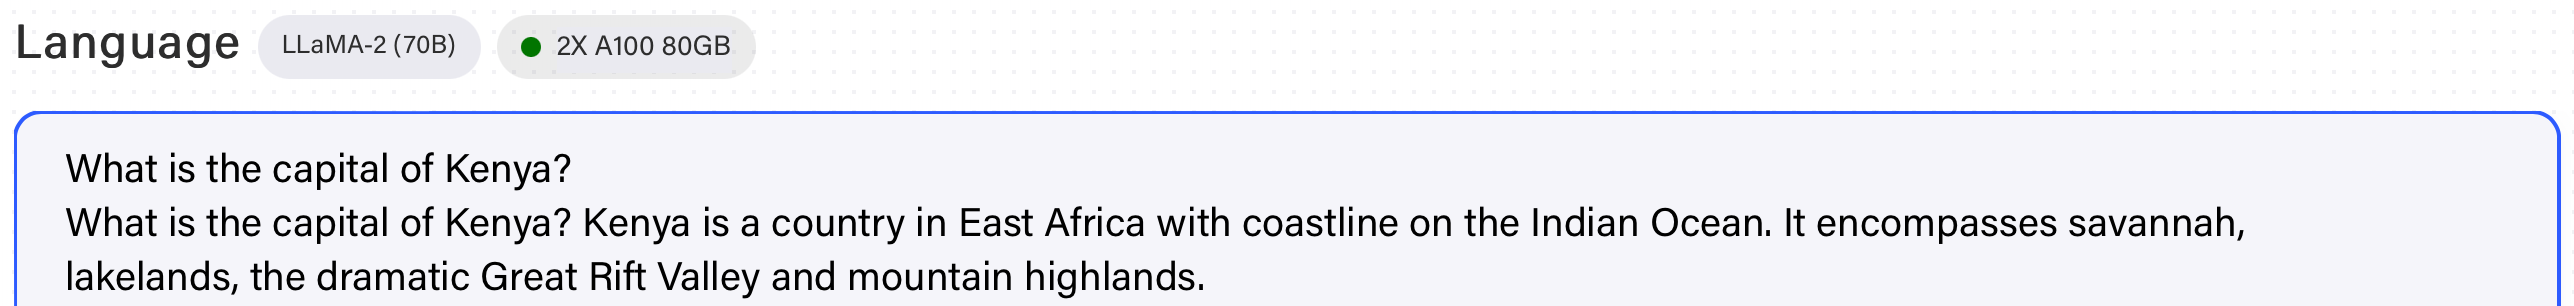
\includegraphics[width=\textwidth]{figures/lm-qa} \\[1em]\pause
        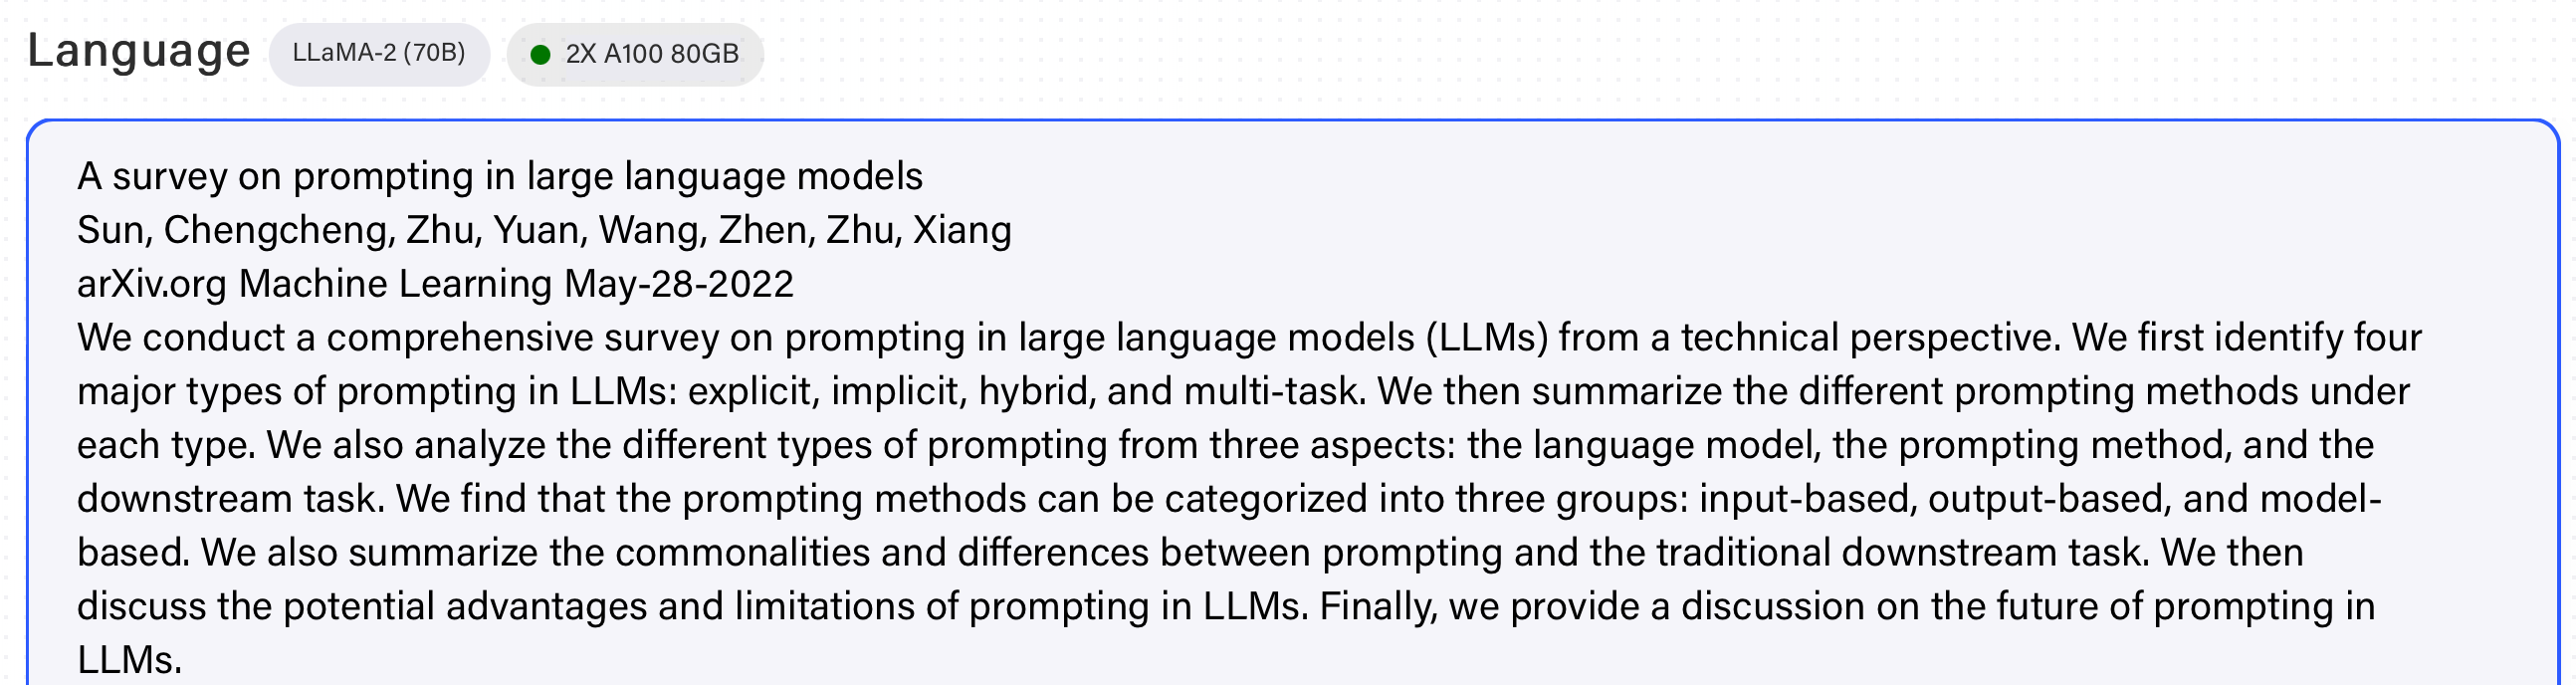
\includegraphics[width=\textwidth]{figures/paper-writing} 
    \end{figure}
\end{frame}

\begin{frame}
    {Early prompting approaches}

    Main goal: adapt the task to a native language modeling task

    Example:\\
    \begin{itemize}
        \item Sentiment classification: [movie review] \blue{This movie is} [great/awful].
        \item Summarization: [document] \blue{TL;DR:} [summary]
    \end{itemize}

    \think{What are potential limitations?}
\end{frame}

\begin{frame}
    {In-context learning}

    How GPT-2 is evaluated on machine translation using GPT-2:
    \begin{wideitemize}
        \item Induce the task through a \blue{demonstration example}:
            $$
                \text{translation} \sim p(\cdot \mid \text{\blue{[french sentence] = [english sentence]}; [french sentence] =})
            $$
        \item WMT-14 French-English test set: 11.5 BLEU (worse than unsupervised MT)
        \item But, there's only 10MB french data in the 40GB training data!
    \end{wideitemize}
\end{frame}

\begin{frame}
    {In-context learning}

    In-context demonstrations elicit target capabilities consistently on GPT-3:\\
    \begin{figure}
        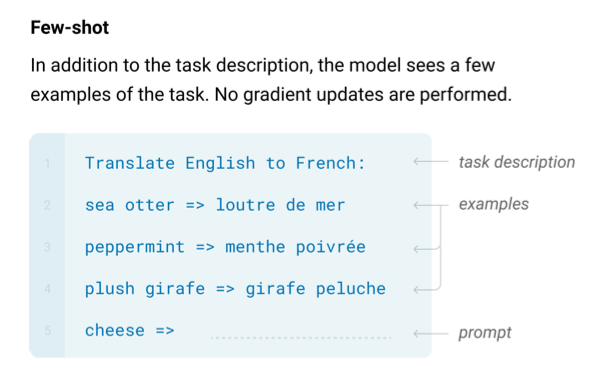
\includegraphics[height=4cm]{figures/icl}
    \end{figure}
    This is surprising as this is not a native language model task!

    Limitations: results can vary with the choice and order of examples \mycite[https://arxiv.org/abs/2102.09690]{[Zhao et al., 2021]}
\end{frame}

\begin{frame}
    {Post-training}
    \begin{wideitemize}
        \item {\bf Goal}: elicit capabilities acquired during pretraining so that the model can be used directly for downstream task, e.g.,
            \begin{itemize}
                \item A chat model that answers user queries
                \item A reasoning model that solves math problems
                \item A shopping assistant that answers questions about products
            \end{itemize}
        \item {\bf Methods}: update the model on some examples of the target task (often require annotation)
            \begin{itemize}
                \item Supervised finetuning (SFT): input and \blue{gold output}
                \item Reinforcement learning (RL): input and an \blue{output judge}
            \end{itemize}
    \end{wideitemize}
\end{frame}

% what does SFT do? not learning new things!

\section{Supervised finetuning}

\begin{frame}
    {Supervised finetuning}
    \begin{columns}
        \begin{column}{0.6\textwidth}
            \begin{itemize}
                \itemsep1em
                \item Supervised learning on the target task
                    \begin{itemize}
                        \item Input: prompt (e.g., instruction or question)
                        \item Output: gold response
                    \end{itemize}
                \item {\bf Key challenge}: {data collection} \\
                    {\em How to get the prompts and responses?}

            \end{itemize}
        \end{column}
        \begin{column}{0.4\textwidth}
        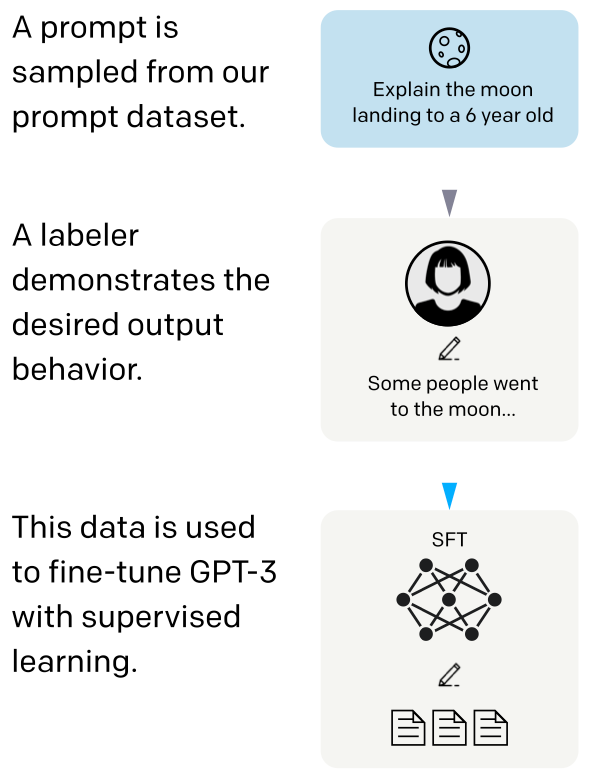
\includegraphics[width=\textwidth]{figures/sft}
        \end{column}
    \end{columns}
\end{frame}

\begin{frame}
    {What kind of data do we need?}
    Idea 1: use existing NLP benchmarks

    \begin{itemize}
        \item \textbf{Natural language inference}:\\
            \textit{
            Suppose "The banker contacted the professors and the athlete". Can we infer that "The banker contacted the professors"?
        }
    \item \textbf{Question answering}:\\
            \textit{
        Given the article "The Panthers finished the regular season [...]", what team did the Panthers defeat?
    }
\item \textbf{Sentiment analysis}:\\
            \textit{
    What's the rating of this review on a scale of 1 to 5:
    We came here on a Saturday night and luckily it wasn't as packed as I thought it would be [...]
}
    \end{itemize}

    \pause
    But this is not what we ask ChatGPT to do! $\quad$ {\bf \red{distribution shift}}
\end{frame}

\begin{frame}
    {What kind of data do we need?}
   
    \begin{columns}
        \begin{column}{0.5\textwidth}
            \begin{itemize}[<+->]
                \item {\bf Problem}: Gap between training and test data 
                \item Straightforward {\bf solution}: collect training data that is similar to test data\\
                    {\em How do we know what test data is like?}
                \item Get some \blue{pilot data}\\
                    {\em which requires a working-ish model first!}
            \end{itemize}
        \end{column}
        \begin{column}{0.5\textwidth}
            \onslide<4->{
                    \begin{tikzpicture}
                        \node (m) {model};
                        \node (r) [below right=1.5cm and 0.5cm of m] {raw data};
                        \node (t) [below left=1.5cm and 0.5cm of m] {training data};
                        \draw[arrow] (m) -- node[above,sloped,anchor=south] {user} (r);
                        \draw[arrow] (t) -- node[above,sloped,anchor=south] {finetuning} (m);
                        \draw[arrow] (r) -- node[above] {annotation} (t);
                    \end{tikzpicture}
                }
        \end{column}
        \end{columns}
\end{frame}

\begin{frame}
    {Data distribution from early OpenAI API}
            \begin{figure}
        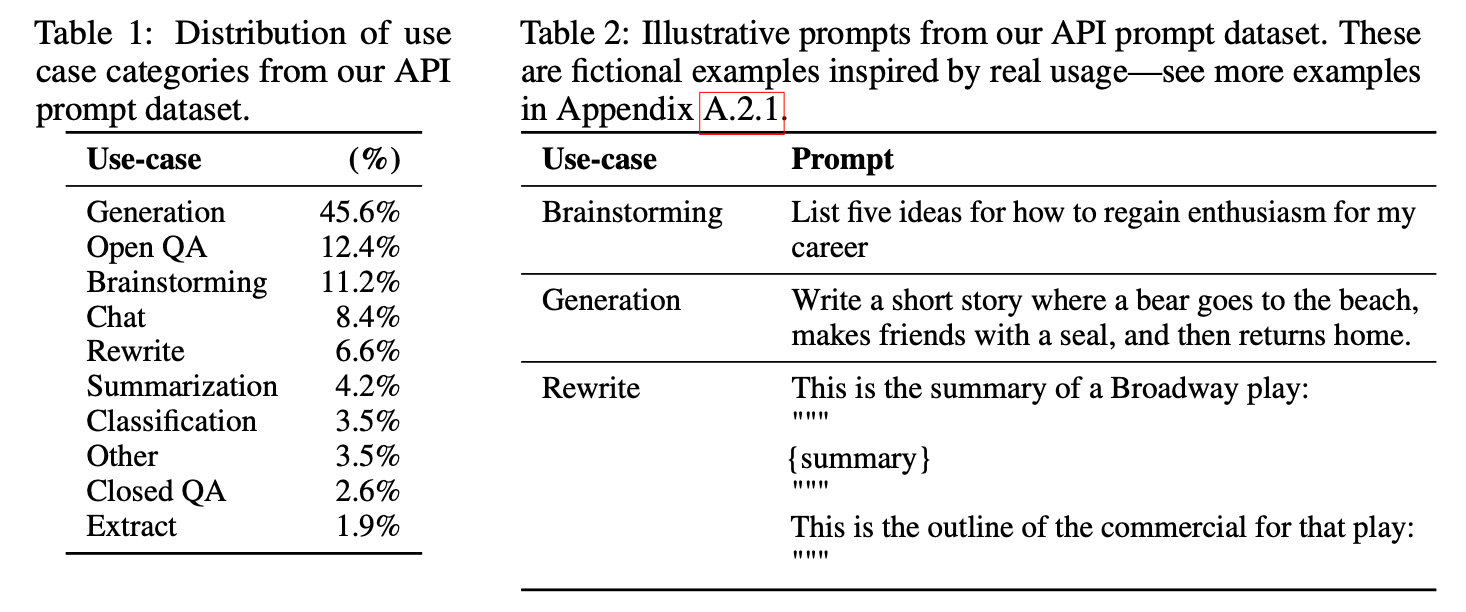
\includegraphics[width=\textwidth]{figures/user-prompt}
            \caption{\mycite[https://arxiv.org/pdf/2203.02155.pdf]{[Ouyang et al., 2022]}}
            \end{figure}
            \pause What if you're not at OpenAI?
\end{frame}

\begin{frame}
    {Synthetic data}
    Use off-the-shelf LMs to generate prompts and responses:\\
    \begin{figure}
        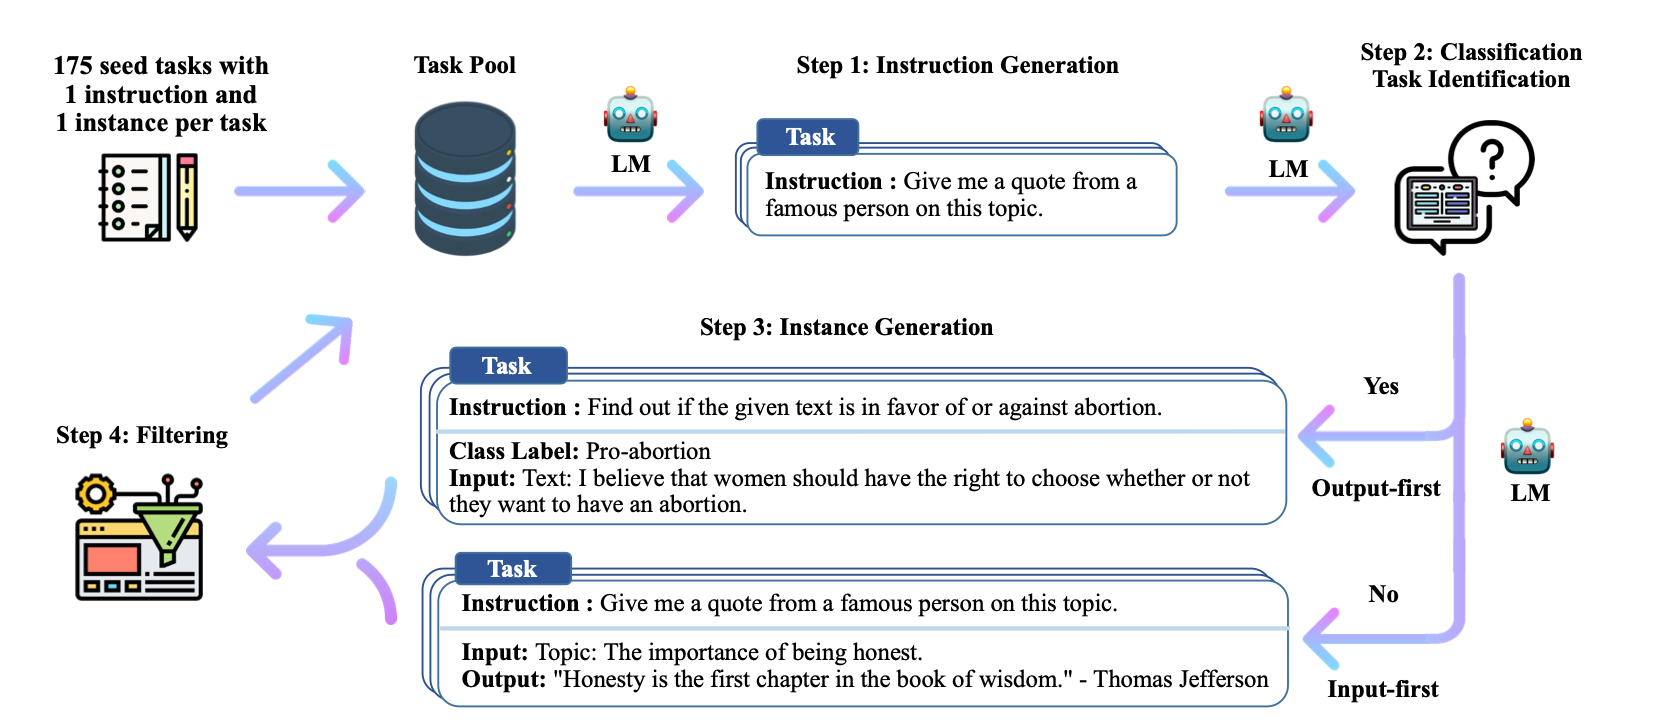
\includegraphics[width=\textwidth]{figures/self-instruct}
            \caption{Self-instruct \mycite[https://arxiv.org/pdf/2212.10560]{[Wang et al., 2023]}}
    \end{figure}
\end{frame}

\begin{frame}
    {The Alpaca model}
    \begin{wideitemize}[<+->]
        \item November 30, 2022: ChatGPT released
        \item February 24, 2023: LLaMA released (open-weight pretrained model)
        \item March 13, 2023: Alpaca released (open-source ChatGPT like model)
            \begin{itemize}[<.->]
                \item 175 seed instruction from Self-Instruct 
                \item 52K prompt-response pair from text-davinci-003 (<\$500)
                \item Supervised finetuning from LLaMA-7B (<\$100)
            \end{itemize}
        \item Impact:
            \begin{itemize}[<.->]
                \item Provides an open-source ChatGPT like model for research
                \item Many later open-source models adopt this distillation approach
            \end{itemize}
    \end{wideitemize}
\end{frame}

\begin{frame}
    {How good are distilled models?}

    \begin{figure}
        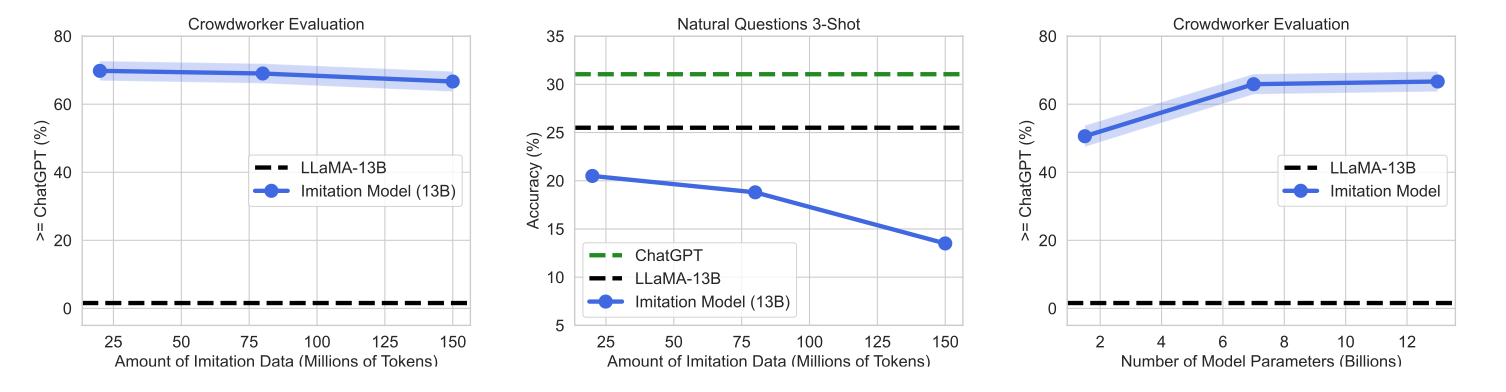
\includegraphics[width=\textwidth]{figures/false-promise}
            \caption{The False Promise of Imitating Proprietary LLMs \mycite[https://arxiv.org/pdf/2305.15717]{[Gudibande et al., 2023]}}
    \end{figure}
    \begin{itemize}
        \item Increasing the amount of synthetic data doesn't keep increasing performance
        \item Distillation can hurt performance on tasks out of the SFT data
        \item Further performance gain comes from stronger pretrained models
    \end{itemize}
\end{frame}

\begin{frame}
    {Parameter efficient finetuning}

    Finetuning all weights of a large model can be expensive (in what way?)

    \pause
    Can we finetune a smaller number of parameters to achieve performance similar to full finetuning?\\
    \begin{itemize}
        \item Select a subset of parameters to update 
            \begin{itemize}
                \item Last k layers \mycite[https://arxiv.org/pdf/1911.03090.pdf]{[Lee et al., 2019]} 
                \item Bias terms (BitFit) \mycite[https://arxiv.org/pdf/2106.10199.pdf]{[Ben-Zaken et al., 2022]}
            \end{itemize}
        \item Add a small number of parameters to adapte the (frozen) pretrained model
            \begin{itemize}
                \item Insert a small MLP in-between layers \mycite[https://arxiv.org/pdf/1902.00751.pdf]{[Houlsby et al., 2019]}
            \end{itemize}
    \end{itemize}
\end{frame}

\begin{frame}
    {Low-rank adaptation of LMs}

    \textbf{LoRA} \mycite[https://arxiv.org/pdf/2106.09685.pdf]{[Hu et al., 2021]}: add low-rank matrices as additional parameters  \\\bigskip

    \begin{columns}
        \begin{column}{0.3\textwidth}
    \begin{figure}
        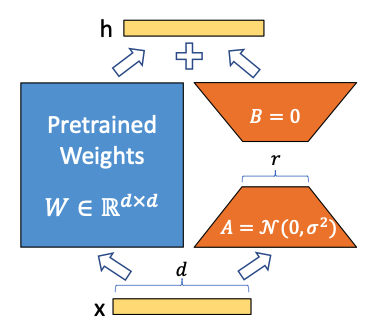
\includegraphics[width=\textwidth]{figures/lora}
    \end{figure}
    \end{column}
        \begin{column}{0.7\textwidth}

            \textbf{Hypothesis}: weight matrices are low rank
            \medskip

            \blue{Adapters}: For any matrix multiplication $h=W_0x$, we modify it to
            $$
            h = W_0x + \blue{\Delta W}x = W_0x + \blue{BA}x
            $$

            \begin{itemize}
                \item $W_0\in\BR^{d\times k}, B\in \BR^{d\times r}, A\in \BR^{r\times k} (r \ll k)$
                \item Initialization: $BA=0$
                \item Can be applied to any weight matrices, e.g., QKV projection matrices
            \end{itemize}
        \end{column}
    \end{columns}
\end{frame}

\begin{frame}
    {Low-rank adaptation of LMs}
    \begin{wideitemize}[<+->]
        \item Converges to full finetuning as $r$ increases and performance goes up consistently
        \item No additional inference latency: $W = W_0 + BA$
        \item Main benefits:
            \begin{itemize}[<.->]
                \item Memory and storage saving (optimizer states, checkpoints): 10,000x reduction on GPT3 ($r=4$)
                \item Easy to switch between different finetuned custom models
            \end{itemize}
    \end{wideitemize}
\end{frame}

% jailbreaking and safety alignment? superficial alignment?

\begin{frame}
    {Summary}
    \begin{wideitemize}
        \item {Supervised finetuning}: train the model on human-annotated prompt-response data 
        \item Data consideration:
            \begin{itemize}
                \item Desiderata: diverse, similar to test data / target task
                \item Often costly to obtain; can synthesize using LMs
            \end{itemize}
        \item Performance upperbound is still decided by the pretrained model
    \end{wideitemize}
\end{frame}

\section{Reinforcement learning}

\begin{frame}
    {Learning from outcomes}
        \textbf{Motivation}:\\
            \begin{itemize}
                \item Demonstrations are expensive to obtain---can we learn from weaker signals?
                \item For many tasks, humans (and animals) only get signal on whether they succeeded or not 
            \end{itemize}

        \textbf{Example}:\\
            \begin{itemize}
                \item Complex physical tasks: learning to shoot a basketball 
                \item Reasoning: learning to play the game of Go 
                \item Decision making: learning to optimize financial portfolios
                \item Communication: learning to articulate your ideas to others
            \end{itemize}
\end{frame}

\begin{frame}
    {Reinforcement learning}

            {\bf Goal}: learning from experience by maximizing the expected cumulative reward\pause
            \begin{enumerate}[<+->]
                \item Agent takes a sequence of \textbf{actions} in a world \hfill \onslide<6->{\blue{\em trial}}\\
                    {\em Get a degree, update CV, apply for a job}
                \item Agent gets \textbf{rewards} along the way indicating how well it did \hfill \onslide<6->{\blue{\em error}}\\
                    {\em No reponse}
                \item Agent updates its \textbf{policy} (on what actions to take) \hfill \onslide<6->{\blue{\em learn}}\\
                    {\em Find a connection? Get an internship? Apply for a different position?}
                \item Go back to 1 \hfill \onslide<6->{\blue{\em rinse and repeat}}
            \end{enumerate}
\end{frame}

\begin{frame}
    {Reinforcement learning: formalization}
    \begin{columns}
        \begin{column}{0.3\textwidth}
        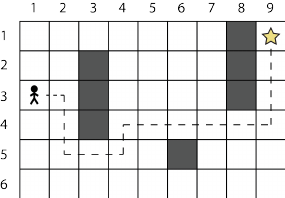
\includegraphics[width=\textwidth]{figures/grid}
        \end{column}
        \begin{column}{0.7\textwidth}
            At each time step $t$, an agent
            \begin{itemize}[<+->]
                \item is in a \textbf{state} $s_t\in\sS$ \hfill($\sS$ is the {\bf state space})\\ \texttt{cell[i][j]} in the grid world
                \item takes an \textbf{action} $a_t\in\sA$ \hfill($\sA$ is the {\bf action space})\\
                    \{\texttt{up, down, left, right}\}
                \item transitions to the next state $s_{t+1}$ according to a {\bf transition function} $p(\cdot\mid s_t, a_t)$\\
                    moves to the corresponding cell if there's no blocker
                \item obtains a {\bf reward} $r(s_t, a_t)$ according to
                    the {\bf reward function} $r\colon \sS \times \sA \rightarrow \BR$\\
                    1 if $s_{t+1}$ is star and 0 otherwise
            \end{itemize}
        \end{column}
    \end{columns}
\end{frame}

\begin{frame}
    {Reinforcement learning: objective}{}
    The agent uses a {\bf policy} $\pi$ to decide which actions to take in a state:\\
    \begin{itemize}
        \item Deterministic: $\pi(s) = a$
        \item Stochastic: $\pi(a\mid s) = \BP(A=a\mid S=s)$ $\quad$ (our focus)
    \end{itemize}
    \pause

    A policy $\pi_\theta$ defines a distribution $p_\theta(\tau)$ over \textbf{trajectories} $\tau=(a_1,s_1,\ldots,a_T,s_T$).
    \vspace{-1em}
    \begin{figure}
        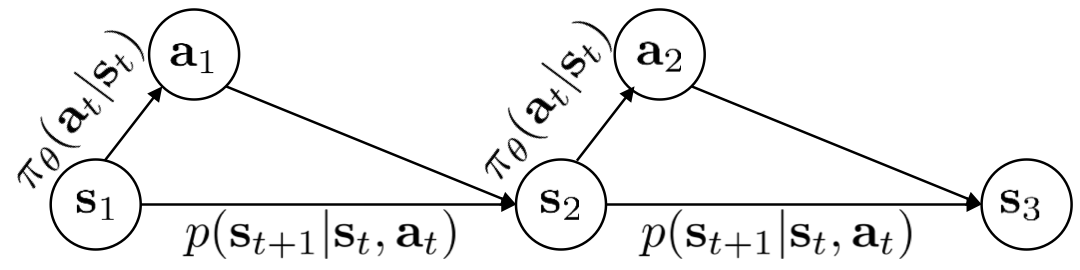
\includegraphics[width=0.5\textwidth]{figures/traj}
    \end{figure}

    \pause\vspace{-1ex}
    The agent's {\bf objective} is to learn a policy $\pi_\theta$ (parametrized by $\theta$) that maximizes the \blue{expected} \green{return}:
    \vspace{-1ex}
    $$
    \mathrm{maximize}\; \blue{\BE_{{\tau\sim p_\theta(\tau)}}} \pb{\green{\sum_{t=1}^T r(s_t, a_t)}}
    $$
\end{frame}

\begin{frame}
    {Sketch of RL algorithms}
    \begin{columns}
        \begin{column}{0.4\textwidth}
            \begin{figure}
        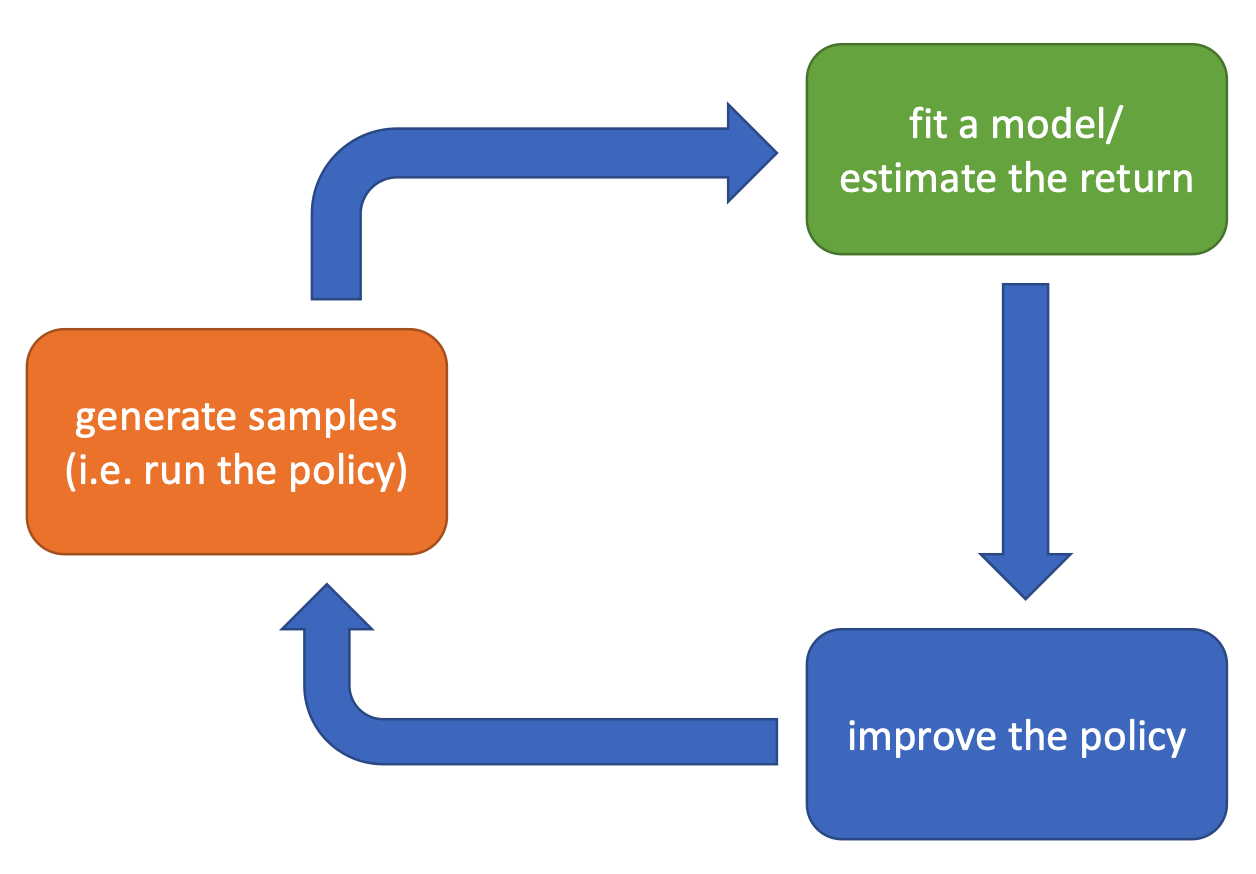
\includegraphics[width=\textwidth]{figures/rl-basics}
                \caption{From Sergey Levine's slides}
            \end{figure}
        \end{column}
        \begin{column}{0.6\textwidth}
            Key steps:\\
            \begin{itemize}
                \item \textcolor{orange}{\bf Trial}: run policy to generate trajectories
                \item \green{\bf Error}: estimate expected return
                \item \blue{\bf Learn}: improve the policy  
            \end{itemize}

            \pause
            Challenges:\\
            \begin{itemize}
                \item Trials could be expensive (e.g., healthcare, education) 
                \item Reward signal could be sparse (e.g., expert feedback) 
                \item May need many samples to learn a good policy
            \end{itemize}
        \end{column}
    \end{columns}
\end{frame}

\begin{frame}
    {Policy gradient algorithms}
            \begin{figure}
        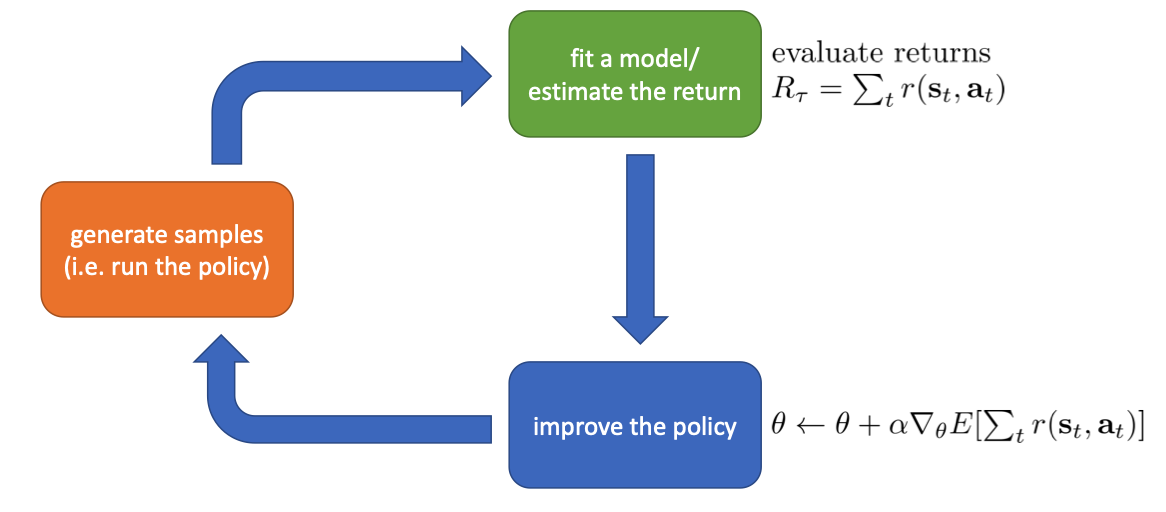
\includegraphics[width=0.8\textwidth]{figures/pg}
            \end{figure}

            \vspace{-2em}
            While not converged\\
            \begin{enumerate}
                \item \textcolor{orange}{Sample trajectories from the current policy }
                \item \green{Estimate return for each trajectories based on observed rewards}
                \item \blue{Take a gradient step on the expected return (w.r.t. the policy)}
            \end{enumerate}
\end{frame}

\begin{frame}
    {How to compute the gradient?}

    Notation: let $r(\tau)=\sum_{t=1}^T r(s_t, a_t)$ be the return.
    \pause

    $$
    \text{Our objective:} \quad
    J(\theta)=\blue{\BE_{\tau\sim p_\theta(\tau)}}\pb{r(\tau)}
    =\blue{\sum_\tau p_\theta(\tau)} r(\tau)
    $$
    \pause

    \begin{columns}
        \begin{column}{0.5\textwidth}
    \begin{align*}
    \nabla_\theta J(\theta) &= \nabla_\theta \sum_\tau p_\theta(\tau) r(\tau)\\
        &= \sum_\tau \green{\nabla_\theta p_\theta(\tau)} r(\tau)\\
        &= \sum_\tau \green{p_\theta(\tau) \nabla_\theta \log p_\theta(\tau)} r(\tau)\\
        &= \BE_{\tau\sim p_\theta(\tau)}\pb{\nabla_\theta \log p_\theta(\tau) r(\tau)}
    \end{align*}
        \end{column}
        \begin{column}{0.5\textwidth}
            \begin{mdframed}[backgroundcolor=gray!20, linewidth=0pt, frametitle={log derivative trick}]
    \begin{align*}
        &p_\theta(\tau) \nabla_\theta \log p_\theta(\tau)\\
        =&   p_\theta(\tau) \frac{\nabla_\theta p_\theta(\tau)}{p_\theta(\tau)}\\
        =& \nabla_\theta p_\theta(\tau)
    \end{align*}
            \end{mdframed}
        \end{column}
    \end{columns}
\end{frame}

\begin{frame}
    {How to compute the gradient?}
    $$
    \nabla_\theta J(\theta) = \BE_{\tau\sim p_\theta(\tau)}\pb{\nabla_\theta \log p_\theta(\tau) r(\tau)}
    \quad \text{Monte Carlo estimation of the expected gradient}
    $$

    \onslide<2->{
    But what is $p_\theta(\tau)$?
    \begin{align*}
        p_\theta(\tau) &= p_\theta(a_1,s_1,\ldots,a_T,s_T) = 
        p(s_1)\prod_{t=1}^T \pi_\theta(a_t\mid s_t) \prod_{t=1}^{T-1}p(s_{t+1}\mid s_t,a_t)\\
        \onslide<3->{
            \log p_\theta(\tau) &= \log p(s_1) + \sum_{t=1}^T \log\pi_\theta(a_t\mid s_t) + \sum_{t=1}^{T-1}\log p(s_{t+1}\mid s_t,a_t)\\
        }
        \onslide<4->{
        \nabla_\theta J(\theta) &= \BE_{\tau\sim p_\theta(\tau)}\pb{
            \p{\sum_{t=1}^T \nabla_\theta\log\pi_\theta(a_t\mid s_t)}
        \p{\sum_{t=1}^T r(s_t,a_t)}
    }}
    \end{align*}
    }
\end{frame}

\begin{frame}
    {Putting everything together}
    REINFORCE algorithm:\\
    \begin{enumerate}
        \item Sample $N$ trajectories $\tau^1,\ldots,\tau^N$ from $\pi_\theta$
        \item Estimate the gradient: 
            $$
            \nabla_\theta J(\theta) \approx \sum_{i=1}^N
            \p{\sum_{t=1}^T \nabla_\theta\log\pi_\theta(a_t^i\mid s_t^i)}
            \p{\sum_{t=1}^T r(s_t^i,a_t^i) }
            $$
        \item Update the policy with gradient ascent: $\theta \leftarrow \theta + \alpha \nabla_\theta J(\theta)$
        \item Go back to 1
    \end{enumerate}
\end{frame}

\begin{frame}
    {How is all this related to LLMs?}{}
    Think of tokens as actions:\\
    \begin{wideitemize}
        \item Action space: vocabulary $\quad$ $a_t = x_t\in\sV$
        \item State space: history / prefix $\quad$ $s_t = (x_1,\ldots,x_{t-1})$
        \item Policy: a language model $\quad$ $p_\theta(x_t\mid x_{<t})$
        \item Trajectory: a sentence / generation $\quad$ $x_1,\ldots,x_T$
    \end{wideitemize}
\end{frame}

\begin{frame}
    {How is all this related to LLMs?}{}
    REINFORCE algorithm on text:\\
    \begin{enumerate}
        \item Sample $N$ generations from the language model $p_\theta$
        \item Estimate the gradient: 
            $
            \hat{g} = \frac{1}{N}\sum_{i=1}^N
            \p{\sum_{t=1}^T \nabla_\theta\log p_\theta(x_t^i\mid x_{<t}^i)}
            r(x_{1:T}) 
            $
        \item Update the policy with gradient ascent: $\theta \leftarrow \theta + \alpha \hat{g}$
        \item Go back to 1
    \end{enumerate}
    \pause

    \begin{mdframed}[backgroundcolor=gray!20, linewidth=0pt, frametitle={What is the algorithm doing?}]
        If $r(x_{1:T})$ is \green{positive}, take a gradient step to \green{increase $p_\theta(x_{1:T})$}.\\ %proportional to the reward.
        If $r(x_{1:T})$ is \red{negative}, take a gradient step to \red{decrease $p_\theta(x_{1:T})$}. %proportional to the reward.

        {\em Supervised learning on model generations weighted by return}
    \end{mdframed}
\end{frame}

\begin{frame}
    {Challenges in policy gradient}
            $$
            \hat{g} = \frac{1}{N}\sum_{i=1}^N
            \p{\sum_{t=1}^T \nabla_\theta\log \pi_\theta(a_t^i\mid s_t^i)}
            \sum_{t=1}^Tr(s_t, a_t) 
            $$
    \begin{wideitemize}[<+->]
        \item We estimate the policy gradient based on a random sample of trajectories\\
            {\it $\hat{g}$ is a random variable}
        \item This estimator is unbiased\\
            {\it In expectation, it is the true policy gradient: $\mathbb{E}[\hat{g}] = \nabla_\theta J(\theta)$}
        \item But it has high variance\\
            {\it Depending on which trajectories we get, $\hat{g}$ can vary greatly}
    \end{wideitemize}
\end{frame}

\begin{frame}
    {Variance of the policy gradient estimator}
            $$
            \hat{g} = \frac{1}{N}\sum_{i=1}^N
            \p{\sum_{t=1}^T \nabla_\theta\log \pi_\theta(a_t^i\mid s_t^i)}
            \sum_{t=1}^Tr(s_t, a_t) 
            $$
    \begin{columns}
        \begin{column}{0.3\textwidth}
        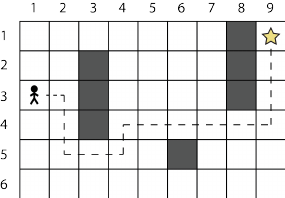
\includegraphics[width=\textwidth]{figures/grid}
        \end{column}
        \begin{column}{0.7\textwidth}
            \begin{wideitemize}
                \item Note that every step along the trajectory is multiplied by the same return
                \item Reward may be sparse and delayed
                \item The {\bf credit assignment} problem: how do we know which step is responsible for the good/bad outcome? 
            \end{wideitemize}
        \end{column}
    \end{columns}
\end{frame}

\begin{frame}
    {Reducing variance: use reward-to-go}

    \begin{wideitemize}
        \item We get a return for the full trajectory $\sum_{t=1}^T r(s_t, a_t)$, how to better allocate it to each step $(s_t, a_t)$?
        \item Future actions ($a_t$) should not affect past rewards ($r_1, \ldots, r_{t-1}$)
        \item $a_t$ only get rewards after $t$, i.e. {\bf reward-to-go}:
            $$
            \hat{g} = \frac{1}{N}\sum_{i=1}^N
            \p{\sum_{t=1}^T \nabla_\theta\log \pi_\theta(a_t^i\mid s_t^i)}
            \sum_{\red{j=t}}^Tr(a_j, s_j) 
            $$
    \end{wideitemize}
\end{frame}

\begin{frame}
    {Important quantities related to reward-to-go}
    \begin{wideitemize}[<+->]
        \item {\bf Q-function}:
                    expected return starting from $s_t$ and taking $a_t$
            $$Q^\pi(s_t, a_t)=r(s_t, a_t) + \BE_{s_{t+1:T}, a_{t+1:T}}\pb{\sum_{t'=t+1}^T r(s_{t'}, a_{t'})}$$
            \begin{itemize}
                \item Reward-to-go: single trajectory estimate of the Q-value from $(s_t, a_t)$
            \end{itemize}

        \item {\bf Value function}: 
                    expected return starting from $s_t$
            $$V^\pi(s_t) = \BE_{a_t\sim\pi(\cdot\mid s_t)}\pb{Q^\pi(s_t, a_t)}$$

        \item Concept check: what is $\BE_{s_1}\pb{V^\pi(s_1)}$?
    \end{wideitemize}
\end{frame}

\begin{frame}
    {Reducing variance: subtract a baseline}

    \begin{wideitemize}[<+->]
        \item Subtract a {\bf baseline} from the return:
            $$
            \hat{g} = \frac{1}{N}\sum_{i=1}^N
            \p{\sum_{t=1}^T \nabla_\theta\log \pi_\theta(a_t^i\mid s_t^i)
            (r(\tau^i) - \blue{b(s_t^i)})}
            $$
            $b(\cdot)$: a function of the state or some constant 
        \item Intuition: the return may not be due to the action you take but just because you are in a state "closer" to the goal %e.g., starting from a state closer to the goal is more likely to get large return regardless of what actions you take
        \item By subtracting a baseline, we measure how much better the action is than the typical return
        \item A simple choice is the average return
            $$
            b(s) = \frac{1}{N}\sum_{i=1}^N r(\tau^i)
            $$
    \end{wideitemize}
\end{frame}

\begin{frame}
    {Reducing variance: subtract a baseline}
    Does this change our objective?\\
    \begin{wideitemize}
    \item $\hat{g}$ is still an {\bf unbiased} estimator, i.e.
    \begin{align*}
        \mathbb{E}\pb{\nabla_\theta\log\pi_\theta(a_t\mid s_t)(r(\tau) - b(s_t))}
        =\mathbb{E}\pb{\nabla_\theta\log\pi_\theta(a_t\mid s_t)r(\tau)}
    \end{align*}
            \vspace{-2em}

            \pause
            \begin{align*}
\mathbb{E}\bigl[\nabla_\theta \log \pi_\theta(a_t \mid s_t)\,b(s_t)\bigr]
&= \mathbb{E}_{s_t}\Bigl[
    b(s_t)\,
    \mathbb{E}_{a_t \sim \pi_\theta(\cdot\mid s_t)}
      \bigl[\nabla_\theta \log \pi_\theta(a_t \mid s_t)\bigr]
\Bigr]
\end{align*}
            \vspace{-2em}

\pause
            \begin{align*}
                \mathbb{E}\pb{\nabla_\theta\log\pi_\theta(a_t\mid s_t)}
                &= \sum_{a_t} \pi_\theta(a_t\mid s_t) \nabla_\theta\log\pi_\theta(a_t\mid s_t)
                = \sum_{a_t} \nabla_\theta \pi_\theta(a_t\mid s_t)\\
                &= \nabla_\theta \sum_{a_t} \pi_\theta(a_t\mid s_t) = \nabla_\theta 1 = 0
            \end{align*}
        \item As long as $b(\cdot)$ does not depend on $a_t$, it doesn't introduce any bias.
    \end{wideitemize}
\end{frame}

\begin{frame}
    {The advantage function}
    \begin{wideitemize}[<+->]
        \item {\bf Advantage function}: how much better $a_t$ is compared to other actions in state $s_t$
            $$
            A^\pi(s_t, a_t) = Q^\pi(s_t, a_t) - V^\pi(s_t)
            $$
            reward-to-go minus a (state-dependent) baseline
        \item How to estimate advantage in policy gradient?
            $$
            \hat{g} = \frac{1}{N}\sum_{i=1}^N
            \p{\sum_{t=1}^T \nabla_\theta\log \pi_\theta(a_t^i\mid s_t^i)}
                    \p{\blue{\sum_{t=1}^Tr(s_t, a_t) - b}}
            $$
            high variance because it's estimated from a single trajectory
        \item We can improve the estimate by sampling more rollouts from $(s_t, a_t)$
        \item Can we fit a function to predict $A^\pi$?
            \begin{itemize}
                \item How does this solve the high variance problem?
            \end{itemize}
    \end{wideitemize}
\end{frame}

\begin{frame}
    {Fitting the value function}
    \begin{wideitemize}[<+->]
        \item Rewrite the advantage function
            \begin{align*}
                A^\pi(s_t, a_t) &= Q^\pi(s_t, a_t) - V^\pi(s_t)\\
                &= r(s_t, a_t) + V^\pi(s_{t+1}) - V^\pi(s_t)
            \end{align*}
        \item So we just need to fit the value function!
        \item Estimate the value from a rollout $\tau^i$
            $$
            \hat{V}^\pi(s^i_t) = \sum_{t'=t}^T r(s^i_{t'}, a^i_{t'})
            $$
        \item This gives us a training example $(s^i_t, \hat{V}^\pi(s^i_t))$
        \item Given a training set $\sD$, train a regression model $w$ by minimizing the squared loss:
            $$
            \sum_{s\in\sD} \p{V^\pi_w(s) - \hat{V}^\pi(s)}^2
            $$
    \end{wideitemize}
\end{frame}

\begin{frame}
    {Actor-Critic methods}
    \begin{itemize}
        \item {\bf Critic}: \blue{evaluate} the policy\\
            update $w$ to improve estimates of $V_w$\\
        \item {\bf Actor}: \blue{improve} the policy\\
            update $\theta$ to improve the policy give feedback from the critic
    \end{itemize}

    \pause
    Algorithm sketch:\\
    \begin{enumerate}
        \item Sample a trajectory from current policy
        \item Update $w$ given the estimated state values
        \item Evaluate $\hat{A}^\pi(s_t, a_t) = r(s_t, a_t) + V^\pi_w(s_{t+1}) - V^\pi_w(s_{t})$
        \item Update the policy with gradient $\hat{g} = \sum_{t=1}^T \nabla_\theta\log\pi_\theta(a_t\mid s_t)\hat{A}^\pi(s_t, a_t)$ 
        \item Go back to 1
    \end{enumerate}
\end{frame}

\begin{frame}{On-Policy vs. Off-Policy}
  \begin{wideitemize}
      \item \textbf{On-Policy} methods use samples from the policy that is currently being optimized (i.e. $\pi_\theta(a\mid s)$).
    \item \textbf{Off-Policy} methods use samples generated by a different behavior policy $\mu(a \mid s)$.
    \item Advantages of off-policy:\pause
    \begin{itemize}
      \item Can reuse old trajectories generated by past policies.
      \item Allows learning from demonstrations or replay buffers.
      \item Can have multiple exploration policies to generate trajectories.
    \end{itemize}
  \end{wideitemize}
\end{frame}
%----------------------------------------

\begin{frame}{Off-Policy Policy Gradient}
  \begin{wideitemize}
    \item Standard on-policy gradient (REINFORCE) is:
    \[
      \nabla_\theta J(\theta)
      \;=\;
      \mathbb{E}_{\tau \sim \pi_\theta}\Bigl[
        \nabla_\theta \log \pi_\theta(\tau)\, r(\tau)
      \Bigr].
    \]
    \item Off-policy scenario: $\tau$ is generated by a behavior policy $\mu(\tau)$, but we want gradient w.r.t. $\pi_\theta$.
    \[
      \nabla_\theta J(\theta)
      \;\neq\;
          \mathbb{E}_{\red{\tau \sim \mu}}\Bigl[
        \nabla_\theta \log \pi_\theta(\tau)
        \,R(\tau)
      \Bigr]
    \]
    \item Key challenge: Correctly handling the discrepancy between $\mu$ and $\pi_\theta$.
  \end{wideitemize}
\end{frame}

\begin{frame}{Importance Sampling: A Quick Review}
  \begin{wideitemize}
    \item We often want an expectation under some distribution $p(x)$,
    but we only have samples from a different distribution $q(x)$.
    \item \textbf{Importance Sampling} uses a correction ratio:
    \[
      \mathbb{E}_{x \sim p}[f(x)]
      \;=\;
      \mathbb{E}_{x \sim q}\Bigl[f(x)\,\frac{p(x)}{q(x)}\Bigr].
    \]
    \item In the RL context:
    \[
      \frac{p(\tau)}{q(\tau)}
      \;\rightarrow\;
      \frac{\pi_\theta(\tau)}{\mu(\tau)}
      %\quad\text{(per step or per trajectory)}.
    \]
    \item This ratio re-weights off-policy trajectories to match the target policy distribution.
  \end{wideitemize}
\end{frame}
%----------------------------------------
\begin{frame}{Off-Policy Policy Gradient}
  \begin{wideitemize}
    \item Off-policy scenario: $\tau$ is generated by a behavior policy $\mu(\tau)$, but we want gradient w.r.t. $\pi_\theta$.
    \[
      \nabla_\theta J(\theta)
      \;=\;
      \mathbb{E}_{\tau \sim \mu}\Bigl[
          \red{\rho(\tau)}
        \,\nabla_\theta \log \pi_\theta(\tau)
        \,R(\tau)
      \Bigr],
      \quad\text{where}\quad
      \rho(\tau)
      \;=\;
      \frac{\pi_\theta(\tau)}{\mu(\tau)}.
    \]
    \item Usually we re-weight per step:
    \[
            \hat{g} = \frac{1}{N}\sum_{i=1}^N
            \p{\sum_{t=1}^T 
            \red{\frac{\pi_\theta(a_t^i\mid s_t^i)}{\mu(a_t^i\mid s_t^i)}} 
            \nabla_\theta\log \pi_\theta(a_t^i\mid s_t^i)}
            \sum_{t=1}^Tr(s^i_t, a^i_t) 
    \]
   \item Importance weight also incurs high variance: when will the ratio blow up?
   \item $\pi_\theta$ and $\mu$ cannot be too different
  \end{wideitemize}
\end{frame}

%----------------------------------------


\begin{frame}
    {Summary}
    \begin{wideitemize}
        \item Reinforcement learning: maximize return through trial and error (rollout, evaluate policy, improve policy)
        \item Policy gradient: increase/decrease likelihood of the trajectory proportionally to the return
        \item Key challenge: gradient is very noisy!
            \begin{itemize}
                \item Use reward-to-go for each action update
                \item Subtract a baseline
                \item Use function approximation for the value/Q function
            \end{itemize}
    \end{wideitemize}
\end{frame}

\end{document}
